\documentclass[12pt,a4paper,titlepage,headinclude,bibtotoc]{scrartcl}

%---- Allgemeine Layout Einstellungen ------------------------------------------

% Für Kopf und Fußzeilen, siehe auch KOMA-Skript Doku
\usepackage[komastyle]{scrpage2}
\pagestyle{plain}
\setheadsepline{0.5pt}[\color{black}]
\automark[section]{chapter}


%Einstellungen für Figuren- und Tabellenbeschriftungen
\setkomafont{captionlabel}{\sffamily\bfseries}
\setcapindent{0em}


%---- Weitere Pakete -----------------------------------------------------------
% Die Pakete sind alle in der TeX Live Distribution enthalten. Wichtige Adressen
% www.ctan.org, www.dante.de

% Sprachunterstützung
\usepackage[ngerman]{babel}

% Benutzung von Umlauten direkt im Text
% entweder "latin1" oder "utf8"
\usepackage[utf8]{inputenc}

% Pakete mit Mathesymbolen und zur Beseitigung von Schwächen der Mathe-Umgebung
\usepackage{latexsym,exscale,stmaryrd,amssymb,amsmath}


\usepackage[nointegrals]{wasysym}
\usepackage{eurosym}

% Anderes Literaturverzeichnisformat
%\usepackage[square,sort&compress]{natbib}
\usepackage{hyperref}
% Für Farbe
\usepackage{color}
\usepackage{graphicx}
\usepackage{wrapfig}
\usepackage{subfigure}

% Caption neben Abbildung
\usepackage{sidecap}

% Befehl für "Entspricht"-Zeichen
\newcommand{\corresponds}{\ensuremath{\mathrel{\widehat{=}}}}
% Befehl für Errorfunction
\newcommand{\erf}[1]{\text{ erf}\ensuremath{\left( #1 \right)}}

%Fußnoten zwingend auf diese Seite setzen
\interfootnotelinepenalty=1000

%Für chemische Formeln (von www.dante.de)
%% Anpassung an LaTeX(2e) von Bernd Raichle
\makeatletter
\DeclareRobustCommand{\chemical}[1]{%
  {\(\m@th
   \edef\resetfontdimens{\noexpand\)%
       \fontdimen16\textfont2=\the\fontdimen16\textfont2
       \fontdimen17\textfont2=\the\fontdimen17\textfont2\relax}%
   \fontdimen16\textfont2=2.7pt \fontdimen17\textfont2=2.7pt
   \mathrm{#1}%
   \resetfontdimens}}
\makeatother

%Honecker-Kasten mit $$\shadowbox{$xxxx$}$$
\usepackage{fancybox}

%SI-Package
\usepackage{siunitx}

%keine Einrückung, wenn Latex doppelte Leerzeile
\parindent0pt

%Bibliography \bibliography{literatur} und \cite{gerthsen}
%\usepackage{cite}
\usepackage{babelbib}
\selectbiblanguage{ngerman}

\begin{document}

\begin{titlepage}
\centering
%\textsc{\Large Praktikum zur Einführung in die physikalische Chemie,\\[1.5ex] Universität Göttingen}

\vspace*{3cm}

\rule{\textwidth}{1pt}\\[0.5cm]
{\huge \bfseries
  V2: Interferenz\\[1.5ex]
  und Wellenlängenmessung}\\[0.5cm]
\rule{\textwidth}{1pt}

\vspace*{3cm}


\begin{Large}
\begin{tabular}{ll}
Durchführende: &  Alea Tokita, Julia Stachowiak\\
Assistentin: & Annemarie Kehl\\
 Versuchsdatum: & 09.11.2015\\
 Datum der Abgabe: & 16.11.2015\\
\end{tabular}
\end{Large}

\vspace*{2.5cm}

\begin{Large}
\fbox{
  \begin{minipage}[t][2cm][t]{6cm} 
   Werte:\\
   $\Delta \lambda = 676 \pm 52 \mathrm {nm} $\\
   $ d \quad = 72 \pm 3 \mathrm{\mu m} $\\
  \end{minipage}
}
\end{Large}

\end{titlepage}

\tableofcontents

\newpage

\section{Theoretische Grundlagen}
Gegeben sind zwei Siebgitter, eines davon mit bekannter und eines mit unbekannter Gitterkonstante. Nacheinander werden sie mit einem Laserstrahl durchleuchtet und das entstehende Interferenzmuster ausgewertet. Ziel des Versuches ist es, daran die Wellenlänge des Lasers und anschließend die unbekannte Gitterkonstante berechnen zu können.

\subsection{Elektromagnetische Wellen}
%\begin{flushleft}
Licht ist elektromagnetische Strahlung, die aus einzelnen Transversalwellen besteht. Diese harmonischen Wellen bewegen sich mit der Lichtgeschwindigkeit $c= 299 792,458 \frac{km}{s}$ durch den Raum. Sie können durch folgende Sinusfunktion in Abhängigkeit des Ortes $x$ und der Zeit $t$ beschrieben werden:
\\
\par %= Leerzeile
\begin{equation}
f(x,t)={ A}\cdot{\sin(kx-wt)}
\end{equation}
\\
\par

Die Wellenzahl $k$ mit $k=\frac{2\pi}{\lambda}$ beschreibt hierbei den Zusammenhang zwischen der Wellenlänge und der Frequenz. \\
Die Relation zu der Periodendauer $T$ gibt die Kreisfrequenz $\omega =\frac{2\pi}{T} $ an.  

%können mit folgender Sinusfunktion in Abhängigkeit zum Ort x beschrieben werden, wobei $\lambda$ die Wellenlänge beschreibt:
%\\
%$f(x)=\sin \frac{2\pi}{\lambda}x $
%\\
%Der Zusammenhang zwischen der Wellenlänge $\lambda$ und deren Frequenz wird mit der Wellenzahl k beschrieben:
%\\
%$k=\frac{2\pi}{\lambda}$

%\end{flushleft} 





%Die Wellenzahl k kann durch folgende Gleichung beschrieben werden:
%\\
 %\centering
%$k= \frac{2\pi}{\lambda}$

\subsection{Phasengeschwindigkeit und Gangunterschied}
Die Ausbreitungsgeschwindigkeit $c$, mit der sich eine Phase einer Welle (der augenblickliche Zustand, z.B. ein Minimum) im Raum fortbewegt, wird als Phasengeschwindigkeit $v$ in Abhängigkeit zu der Frequenz $v=\frac{1}{T}$ und der Wellenlänge $\lambda$ beschrieben:\\
\par
\begin{equation}
\vec{v}_p = {v}\cdot{\lambda}
\end{equation}
\\
\par

Phasengeschwindigkeit und Gangunterschied werden in Abbildung 1 verdeutlicht.

\begin{figure} [h]
\begin{center}
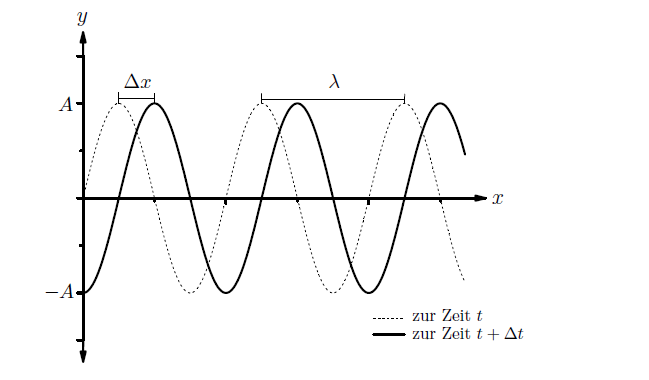
\includegraphics[scale=0.75]{Phasengeschwindigkeit2.png} \end{center}
\caption{Phasengeschwindigkeit und Gangunterschied}
\end{figure}
%Achtung: hier Phasengeschwindigkeit als c

Werden zwei Wellen mit gleicher Phasengeschwindigkeit zeitlich verzögert ausgesandt, so ergibt sich eine Wegdifferenz $\Delta x$, der sogenannte Gangunterschied $\delta$. 

\subsection{Interferenz}
Überlagern sich zwei oder mehr Wellen, so führt dies zu einer Amplitudenänderung. Die Wellen verschmelzen zu einer neuen Welle mit größerer oder kleinerer Amplitude, je nachdem, ob gleiche oder unterschiedliche Phasen aufeinandertreffen. Diese Erscheinung nennt man Interferenz. Treffen Maxima oder Minima aufeinander, so wird die Amplitude verstärkt (konstruktive Interferenz); trifft Maximum auf Minium so löschen sich die Wellen gegenseitig aus (destruktive Interferenz). 
Eine konstruktive Interferenz zweier Wellen ist demnach nur möglich, wenn der Gangunterschied ebendieser ganzzahliges Vielfaches der Wellenlänge ist:\\
\par
\begin{equation}
\delta={n}\cdot {\lambda} \quad \mathrm{mit}\quad n = 0,1,2...
\end{equation}
\\
\par

Ist $\delta$ jedoch ein ungradzahliges Vielfaches der halben Wellenlänge, so tritt destruktive Interferenz auf. \\
\par
\begin{equation}
\delta = \frac{(2n+1)\lambda}{2} \quad \mathrm{mit}\quad  n=0,1,2...
\end{equation}
\\
\par


\subsection{Streuung und Beugung}
Trifft eine Welle auf ein Hindernis, so verändert sie ihren geometrisch vorgeschriebenen Weg, dh. sie wird gestreut. %Der Begriff Streuung ist ein Sammelbegriff für viele physikalische Phänomene wie Reflexion, Brechung, Beugung etc., bei denen die Welle außerdem ihre Phase und Wellenlänge $\lambda$ verändern kann. 
Trifft ein Wellenzug senkrecht auf ein Gitter mit der Gitterkonstante $d$, so werden seine verschiedenen Wellen an benachbarten Gitterstäben unter dem Beugungswinkel $\beta_n$ gebeugt. Konstruktive Interferenz ergibt sich nur, wenn (5) zutrifft, dh. der Gangunterschied $\delta$ ein ganzzahliges Vielfaches von $\lambda$ beträgt.

\begin{figure} [h]
\begin{center}
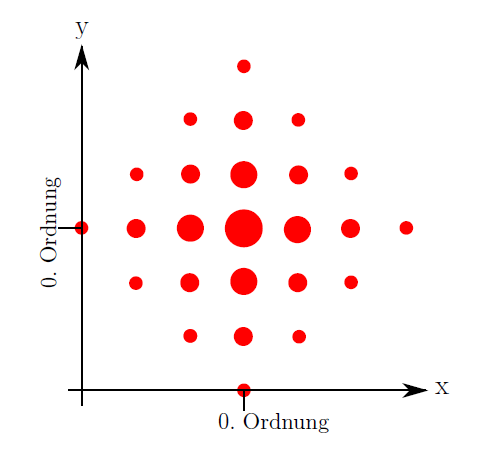
\includegraphics[scale=0.5]{Beugungsbild.png} \end{center}
\caption{Auf den Schirm abgebildetes Beugungsbild}
\end{figure}

Bei Abbildung des entstehenden Musters (Abbildung 2) auf einen Schirm wird ein Beugungsbild der Wellen mit konstruktiver Interferenz sichtbar. Die Beugungsordnung beschreibt, an welcher Gitterebene die Welle gebeugt wurde. 

\begin{figure} [h]
\begin{center}
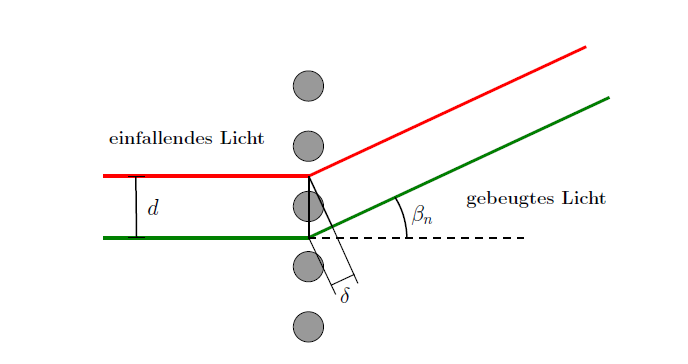
\includegraphics[scale=0.65]{Gangunterschied.png} \end{center}
\caption{Entstehung des Gangunterschiedes $\delta$ bei Beugung an einem Gitter}
\end{figure}

\section{Experimentelles}

\subsection{Versuchsaufbau}

\subsubsection{Skizze der Apparatur}
\begin{figure} [h]
\begin{center}
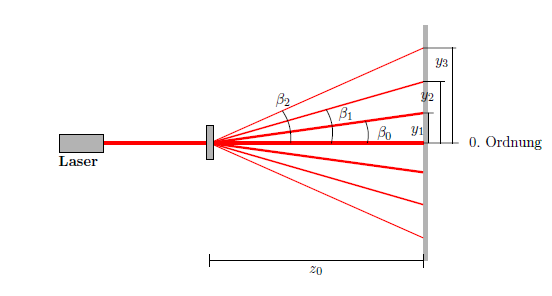
\includegraphics[scale=1]{Versuchsaufbau.png} \end{center}
\caption{Versuchsaufbau}
\end{figure}

Zunächst wird der Versuch wie auf der Skizze beschrieben aufgebaut.
Ein Laser strahlt auf ein Siebgitter, wodurch auf einem sich dahinter befindenden, an ein Holzrahmen befestigtes, Millimeterpapier ein Interferenzmuster entsteht. Anschließend wird das Siebgitter durch ein anderes Siebgitter, nun unbekannter Gitterkonstante, ersetzt.


\subsection{Durchführung}
Die entstehenden Beugungsmuster werden auf das Papier übertragen. Dabei werden jeweils die drei Punkte  oberhalb und unterhalb des nullten Beugunsmaximum übertragen.
Nach Übertragung der Punkte werden die Millitmeterpapiere von dem Holzrahmen genommen und die Abstände $y_{y},y_{2},y_{3}$ der Punkte oberhalb des nullten Maximum zu diesem und die Abstände $y_{-1},y_{-2},y_{-3}$ unterhalb des nullten Maximum zu diesem gemessen. Außerdem wird der Abstand $z_{o}$ vom Laser zum Holzrahmen gemessen.


\section{Messwerte}

\begin{table} [h]
\centering
\begin{large}

\end{large}
\begin{tabular}{|p{4 cm}||p{4 cm}|p{4 cm}|}
        \hline
          Abstand  & Gitter 1  & Gitter 2 \\
          in mm & d=50,1$\mu$m & d unbekannt\\
         \hline 
         $y_3 $& 28 & 16 \\
         \hline
         $y_2 $& 19 & 11\\
         \hline
         $y_{1} $& 9,0 & 6 \\
         \hline
         $y_{-1}$& 9,0 & 5 \\
         \hline
         $y_{-2}$& 18 & 11 \\
         \hline             
         $y_{-3}$& 28 & 17 \\
         \hline
\end{tabular}
\end{table}



Abstand Laser- Holzrahmen: $z_0$ = 70 cm



\section{Auswertung}

Die auf dem Schirm abgebildeten Punkte bilden die Beugungsebenen nullten bis 3. bzw. -3. Grades unterhalb und oberhalb der nullten Ebene. Die Abstände der Punkte oberhalb und unterhalb der nullten Beugunsebene ergeben die Strecke $y_n$. $z_0= 0,7 m$ beschreibt den Abstand zwischen Laser und Holzrahmen. 

\begin{figure} [h]
\begin{center}
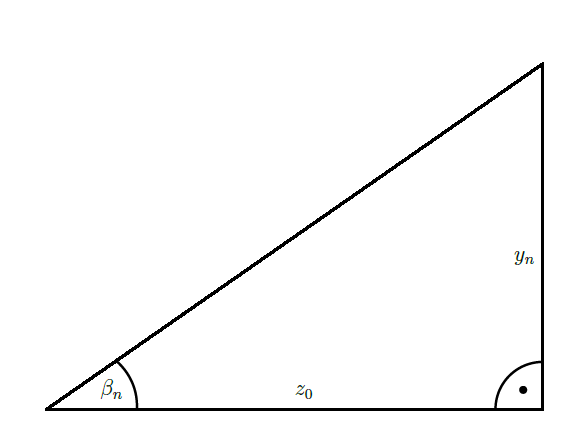
\includegraphics[scale=0.4]{Dreieck.png} \end{center}
\caption{Beugungswinkel $\beta_n$ im Verhältnis zu $z_0$ und $y_n$}
\end{figure}

Es ergibt sich ein rechtwinkliges Dreick (Abildung 5), sodass die Begungswinkel $\beta_n$ zu errechnen sind:

\begin{equation}
\beta_n = arctan(\frac{y_n}{z_0})
\end{equation}

\par

Somit ergeben sich für die Winkel folgende Werte: 

\begin{table} [h]
\centering
\begin{tabular}{|p{4 cm}||p{4 cm}|}
        \hline
		n& $\beta_n$\\
         \hline 
         $3$ & $2,291^\circ$  \\
         \hline
         $2$ & $1,555^\circ$\\
         \hline
         $1$ & $0,737^\circ$ \\
         \hline
         $-1$ & $0,737^\circ$ \\
         \hline
         $-2$ & $1,473^\circ$ \\
         \hline             
         $-3$ & $2,291^\circ$ \\
         \hline
\end{tabular}
\end{table}

Wie auf Abbildung 3 ersichtlich, ergibt sich ein zweites Dreieck mit dem gleichen Winkel $\beta_n$, dessen Seitenlängen die (für das erste Gitter bekannte) Gitterkonstante $d= 50,1\mu=50,1\cdot10^{-6}m$, als auch den unbekannten Ganunterschied $\delta$ zeigen. Damit ist folgende Formel aufgestellt:

\begin{equation}
\sin{\beta_n}=\frac{\delta}{d}\cdot n
\end{equation}

Damit die Wellen konstruktiv miteinander interferieren können, muss der Gangunterschied $\delta$ ein ganzzahliges Vielfaches von $\lambda$ betragen und kann somit mit $\lambda$ gleichgesetzt werden. Durch Umstellen der Gleichung nach $\delta$ bzw. $\lambda$ ergibt sich folgende Formel:

\begin{equation}
\lambda = \frac{d\cdot \sin\beta_n}{|n|}
\end{equation}

Für die Wellenlängen ergeben sich so folgende Werte:

\begin{table} [h]
\centering
\begin{tabular}{|p{4 cm}||p{4 cm}|}
        \hline
		n& $\lambda$ in m\\
         \hline 
         $3$ & $6,676\cdot10^{-7}$  \\
         \hline
         $2$ & $6,789\cdot10^{-7}$\\
         \hline
         $1$ & $6,444\cdot10^{-7}$ \\
         \hline
         $-1$ & $6,444\cdot10^{-7}$ \\
         \hline
         $-2$ & $6,440\cdot10^{-7}$ \\
         \hline             
         $-3$ & $6,676\cdot^{-7}$ \\
         \hline
\end{tabular}
\end{table}

Zur Berechnung des Mittelwertes wird folgende Formel angewandt:

\[\bar{x} =\frac{1}{N}\sum_{i=1}^n x_i\] mit N=6

Somit ergibt sich für $\bar{x} = 6,580\cdot10^{-7} m $

\subsection{Bestimmung von $\lambda$ aus der Auftragung}

Nach Gleichung 6 ergibt sich:

\begin{equation}
\sin\beta_n = \frac{n}{d}\cdot \lambda
\end{equation}

Nach der Allgemeinform für lineare Gleichungssysteme ergibt sich hieraus somit $\lambda$ als Steigung und kann der Auftragung entnommen werden. Somit werden für ${lambda}$ gegen $\frac{|n|}{d}$ folgende Werte aufgetragen:

\begin{table} [h]
\centering
\begin{tabular}{|p{4 cm}||p{4 cm}|p{4 cm}}
        \hline
		n & $\sin(\beta_n)$ & $\frac{|n|}{d}$\\
         \hline 
         $3$ & 0,4 & 59880 m  \\
         \hline
         $2$ & 0,28 & 39920 m \\
         \hline
         $1$ & 0,013 & 19960 m\\
         \hline
         $-1$ & 0,013 &    \\
         \hline
         $-2$ & 0,026 &    \\
         \hline             
         $-3$ & 0,04 &    \\
         \hline
\end{tabular}
\end{table}

Aus dem Steigungsdreieck in der Auftragung ergibt sich somit für $\lambda$ :

\begin{equation}
\lambda =  \frac{\Delta \sin(\beta_n)}{\Delta\frac{n}{d}} = \frac{0,04 - 0,013}{59880 - 19960} = 6,764 \cdot 10^{-7} m
\end{equation}

Daraus lässt sich die Gitterkonstante errechnen und mit folgender Formel ergeben sich folgende Werte:

\begin{equation}
d = \dfrac{n\cdot \lambda}{\sin(\beta_|n|)} \quad \mathrm{mit}\quad n= 1 
\end{equation}

\begin{table} [h]
\centering
\begin{tabular}{|p{4 cm}||p{4 cm}|}
        \hline
		n & d \\
         \hline 
         $3$ & $8,81\cdot 10^{-5}$  \\
         \hline
         $2$ & $8,44 \cdot 10 ^{-5}$ \\
         \hline
         $1$ & $7,88\cdot 10^{-5}$\\
         \hline
         $|-1|$ & $9,46 \cdot 10^{-5} $   \\
         \hline
         $|-2|$ & $8,44\cdot 10^{-5}  $  \\
         \hline             
         $|-3|$ & $8,44\cdot 10^{-5}$   \\
         \hline
\end{tabular}
\end{table}

Für den Mittelwert ergibt sich:
$\bar{d} = 8,58\cdot 10^{-5}$

\subsection{Bestimmung von d aus der Auftragung}

Bei einer Auftragung von $\sin_\beta $ gegen $n \cdot \lambda $ ergibt sich d als Steigung (siehe Formel 10). 
Nach Formel 5 ergeben sich für $\beta_n$ folgende Werte:

\begin{table} [h]
\centering
\begin{tabular}{|p{4 cm}||p{4 cm}|}
        \hline
		n & $\beta_n$ \\
         \hline 
         $3$ & $1,309^\circ$  \\
         \hline
         $2$ & $0,900^\circ$ \\
         \hline
         $1$ & $0,491^\circ$\\
         \hline
         $-1$ & $0,490^\circ$   \\
         \hline
         $-2$ & $0,900^\circ$  \\
         \hline             
         $-3$ & $1,391^\circ$   \\
         \hline
\end{tabular}
\end{table}

Daraus errechnet sich der $\sin_n$:

\begin{table} [h]
\centering
\begin{tabular}{|p{4 cm}||p{4 cm}|}
        \hline
		n & $\sin(\beta_n)$ \\
         \hline 
         $3$ & $0,023$  \\
         \hline
         $2$ & $0,016$ \\
         \hline
         $1$ & $0,008569$\\
         \hline
         $-1$ & $0,007138$   \\
         \hline
         $-2$ & $0,016$  \\
         \hline             
         $-3$ & $0,024$   \\
         \hline
\end{tabular}
\end{table}

Somit ergibt sich für $d$ aus der Auftragung:

$ d= \frac{\Delta n \cdot \lambda}{\Delta \sin(\beta_n]} = 7,2\cdot 10^{-5} = 72\mu m $

\par
\par
\par



\section{Fehlerrechnung}
\subsection{Fehlerfortpflanzung}
Im Versuch entstehen Fehler, sowohl durch die Messungen mit dem Zollstock als auch bei der Übertragung und Ausmessen der Werte auf dem Millimeterpapier. Messungenauigkeiten beim Messen mit dem Zollstock entstehen dadurch, dass es schwierig ist, den Zollstock exakt so anzulegen, dass die kürzeste Strecke zwischen Holzrahmen und Laser gemessen wird, auch ist die Skalierung nur auf einen Millimeter genau gegeben. Wir gehen daher von folgendem Fehler aus: $\Delta_{Zollstock}={2} \cdot{10^{-2}}m$. Die Messungenauigkeiten bezüglich des Millimeterpapiers entstehen durch ungenaue Übertragung, etwa sind die Laserpunkte eher in Tropfenform, sodass der Mittelpunkt nicht exakt bestimmt werden kann, des weiteren ist die Messung der Abstände nur auf Millimeter genau. $\Delta_{Millimeterpapier}={2} \cdot {10^{-3}}$ \\

Diese Fehler setzten sich nun in den weiteren Berechnungen fort. Zunächst lassen sich mithilfe der Gaußschen Fehlerfortpflanzung maximale und minimale Werte mithilfe folgender Formel für die erste Berechnung des Winkels $\beta$ errechnen:\\

\begin{equation}
\Delta \beta = \sin( \quad \sqrt{({\dfrac{1}{y_{|n|}^{2}+z_{0}^{2}}} \cdot {{2} \cdot {10^{-3}}})^{2} + (- {\dfrac{1}{y_{|n|}^{2}+z_{0}^{2}}} \cdot {{2} \cdot {10^{-2}}})^{2}} \quad)
\end{equation}\\\\\

Es ergeben sich die folgenden Werte: \\\\\\\\\\\\
   
\par


\begin{table} [h]
\centering
\begin{tabular}{|p{2 cm}||p{3 cm}|p{3 cm}|p{3 cm}|}
		\hline
         n & $\sin\beta_n$  & $\sin\beta_max $ & $sin\beta_min$ \\
         \hline 
         $1 $& 0,013& 0,01357 & 0,01215 \\
         \hline
         $2 $& 0,028&  0,03241 &0,0218 \\
         \hline
         $3 $& 0,04& 0,04054& 0,0394\\
         \hline
         $-1$& 0,013&  0,01357& 0,0122 \\
         \hline
         $-2$& 0,026& 0,02641 & 0,02499 \\
         \hline             
         $-3$& 0,04& 0,04054  & 0,0394 \\
         \hline
\end{tabular}
\end{table}

\begin{flushleft}
Diese Werte lassen sich nun in der Auftragung von $ \beta_{|n|} $ gegen $ \frac{|n|}{d} $ als Fehlerbalken einzeichnen. Durch einzeichnen einer Ausgleichsgeraden ergibt sich eine minimale und maximale Steigung von $ \lambda $.\\

$ \lambda_{max} = 693 \mathrm {nm} $\\
$ \lambda_{min} = 589 \mathrm {nm} $\\


Daraus lässt sich nun der Absolute Fehler mithilfe folgender Formel berechnen:\\

$ \Delta \lambda = \dfrac{ \lambda_{max}-\lambda_{min}}{2}= \pm 52 \mathrm {nm} $\\

Der Fehler von $ \Delta \lambda $ lässt sich nun in Form von Fehlerbalken in die zweite Auftragung zur Bestimmung von \emph{d} eintragen. Es ergeben sich folgende Werte für die Fehlerbalken:

\begin{table} [h]
\centering
\begin{tabular}{|p{6 cm}|p{6 cm}|}
		\hline
         Obere Grenze des Fehlerbalkens: & Untere Grenze des Fehlerbalkens: \\
         
         $ {|n|} \cdot {\lambda_{max}} $ & $ {|n|} \cdot {\lambda_{min}} $ \\
         \hline
         ${0,69} \cdot {10^{-6}} $& ${0,59} \cdot {10^{-6}} $ \\
         \hline
         ${1,4} \cdot {10^{-6}} $& ${1,2} \cdot {10^{-6}} $\\
         \hline
         ${2,1} \cdot {10^{-6}} $&${1,8} \cdot {10^{-6}} $ \\
         \hline
\end{tabular}
\end{table}
 
In diese Auftragung lässt sich wieder eine Ausgleichsgerade maximaler und minimaler Steigung zeichnen und so ein maximaler und minimaler Wert für \emph{d} ermitteln:
$ d_{max} = 76 \mathrm{\mu m} $\\
$ d_{min} = 70 \mathrm{\mu m} $\\
Der Absolute Fehler wird nun wie folgt berechnet:
$ \Delta d = \dfrac{ d_{max}-d_{min}}{2}= \pm 3 \mathrm {\mu m} $\\
\end{flushleft}

\subsection{Diskussion systematischer Fehler}
Im Versuch können zunächst systematische Fehler beim Abmessen der Längen auftreten. Etwa könnte der Zollstock oder das Geodreieck fehlerhaft sein und immer zu kleine oder zu große Längen messen. Des weiteren ist auch der Laser fehlerhaft, in dem Sinne, dass nicht nur Licht einer bestimmten Wellenlänge ausgesandt wird sondern die Wellenlänge ein wenig variiert. Dadurch kommt es beim Beugungsmuster zu tropfenförmigen anstelle von runden Lichtpunkten. Hier muss darauf geachtet werden, einheitlich an einer Stelle des jeweiligen Tropfens zu messen.

  
\subsection{Vergleich mit Literaturwerten}

Für die Wellenlänge erhalten wir aus der Auftragung folgendes Ergebnis:\\
\begin{center}
$\Delta \lambda = 676 \pm 52 \mathrm {nm} $\\
Herstellerangabe $ \Delta \lambda = 630-680 \mathrm {nm} $\\
\end{center}

Die gemessene Wellenlänge liegt im Bereich der Herstellerangaben. Die Fehlergrenzen weichen ein wenig von den Fehlergrenzen der Herstellerangabe ab.\\\\

Für die Gitterkonstante erhalten wir, ebenfalls aus der Auftragung, folgenden Wert:\\\\
\centering
$ d = 72 \pm 3 \mathrm{\mu m} $\\

\begin{flushleft}
Für die Gitterkonstante liegen keine Herstellerangaben vor. Jedoch ist die Gitterkonstante des ersten Gitters mit $d = 50,1 \mathrm{\mu m} $ vom Hersteller gegeben. Bei dem Vergleich der Beugungsmuster ist aufällig, dass die Punkte bei dem zweiten Gitter enger aneinander liegen, was bedeutet, dass es sich um ein Gitter mit einer größeren Gitterkonstante handeln muss. Da sich dies im Vergleich unseres Wertes, auch mit den Fehlergrenzen, mit dem Herstellerwert bestätigen lässt, stimmt unser Wert mindestens in dieser Beziehung.
\vspace{1cm}
Indem man Fehler minimiert lassen sich noch genauere Ergebnisse, die auch mit den Herstellerangaben besser übereinstimmen. So könnte man etwa anstelle des doch eher ungenauen Zollstock und Geodreiecks etwa eine Schieblehre verenden und mit einem Winkelmesser den Abstand zwischen Laser und Holzrahmen exakter bestimmen. Mit einem Laser, der nur Licht einer Wellenlänge aussendet, könnte man die Punkte des Beugungsmuster genauer übertragen. Dies würde ebenfalls durch einen fest installierten Holzrahmen vereinfacht werden.
\end{flushleft}

\section{Literaturverzeichnis}
\begin{flushleft}
1 \quad Gerd Wedler: Lehrbuch der physikalischen Chemie, 5. Aufl., WILEY-VCH Verlag GmbH Co. KGaA, Weinheim,2004, Seite 109-130.\\
2\quad Götz, Eckhold: Sriptum zur Einführung in die physikalische Chemie, Institut für physikalische Chemie, Uni Göttingen, 2015 Seite 14-18.\\
3 \quad Skriptum für das Praktikum zur Einführung in die Physikalische Chemie, Institut für physikalische Chemie, Uni Göttingen, 2015, Seite 1-12.\\
\end{flushleft}






\end{document}


